\section{Resultate
	\label{ableitung:section:resultate}}
\rhead{Resultate}
Dei Resultate dieser Arbeit sollen hauptäschlich zeigen, ob die Finite Differenzen Methode als Option zur Optimierung neuronaler Netzwerke geeignet ist. Es ist klar, dass implementationsbedingt die Trainingsgeschwindigkeit nicht dem Backpropagation Algorithmus das Wasser reichen kann. Viel wichtiger ist eine qualitative Aussage treffen zu können, ob die Methode eine interessante Variante darstellt und ob das Gedankenexperiment funktioniert.

Um dies an einem einfachen Beispiel zu verdeutlichen, wird versucht eine logische XOR Verknüpfung zu trainieren. Ein XOR-Gate ist ein elektronisches Bauteil, welches im Prinzip eine 'Entweder-Oder' Logik abbildet. Im gewählten Fall hat das Bauteil 2 digitale Eingänge und sollte entweder der Erste oder der Zweite aktiv sein, so ist der Ausgang ebenfalls aktiv. Sollte keiner der beiden Ausänge oder beide Ausgänge aktiv sein, so ist der Ausgang inaktiv. Dies kann man der Logiktabelle in Abbildung \ref{ableitung:fig:xor-gate-logic} entnehmen. \textit{Anmerkung: Wie zum Teufel wird das GATE gefixed, Linien nicht parallel!}

\begin{figure}[h]
	 \centering
\begin{tabular}{cc}
	\begin{tikzpicture}
	
	\node (x1) at (0, 0.95) {$x_1$};
	\node (x2) at (0, 1.05) {$x_2$};
	\node (y) at (3, 1) {$y$};
	
	\node[xor gate US, draw, logic gate inputs=nn] at (1.5, 1) (notx) {};
	
	\draw (x1) -- (notx);
	\draw (x2) -- (notx);

	\draw (notx.output) -- (y);
	
	
	\end{tikzpicture}	
	&
	\begin{tabular}{cc|c}
		\hline
		$x_1$ & $x_2$ & $y$ \\
		\hline
		0 & 0 & 0 \\ 
		0 & 1 & 1 \\ 
		1 & 0 & 1 \\ 
		1 & 1 & 0 \\
		\hline						
	\end{tabular}
\end{tabular}
	\caption{Das XOR-Gate und die dazugehörige Logiktabelle}
	\label{ableitung:fig:xor-gate-logic}
\end{figure}
\tikzstyle{inputNode}=[draw,circle,minimum size=17pt,inner sep=0pt]
\tikzstyle{stateTransition}=[-stealth, thick]
\begin{figure}
	\centering
	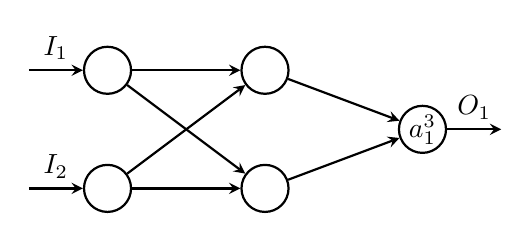
\begin{tikzpicture}
	
	\node[inputNode, thick] (i1) at (5, 1.5) {};
	\node[inputNode, thick] (i2) at (5, 0) {};
	
	\node[inputNode, thick] (h1) at (7, 1.5) {};
	\node[inputNode, thick] (h2) at (7, 0) {};
	
	\node[inputNode, thick] (o1) at (9, 0.75) {$a^{3}_{1}$};
	
	\draw[stateTransition] (4, 1.5) -- node[above] {$I_1$} (i1);
	\draw[stateTransition] (4, 0) -- node[above] {$I_2$} (i2);
	
	
	\draw[stateTransition] (i1) -- (h1);
	\draw[stateTransition] (i1) -- (h2);
	\draw[stateTransition] (i2) -- (h1);
	\draw[stateTransition] (i2) -- (h2);
	
	\draw[stateTransition] (h1) -- (o1);
	\draw[stateTransition] (h2) -- (o1);
	
	\draw[stateTransition] (o1) -- node[above] {$O_1$} (10, 0.75);

	\end{tikzpicture}
	\caption{Das Neuronale Netzwerk zum erlernen des XOR Logikoperators}
	\label{ableitung:fig:nn-result-net}
\end{figure}
Das gewählte Netzwerk, um diese Logik abzubilden, besteht aus 3 Schichten und ist in Abbildung \ref{ableitung:fig:nn-result-net} ersichtlich. Die Mittelschicht (Hidden Layer) wird benötigt, da sich mit nur einer Schicht keine Funktion finden lässt welche die Punkte in einer Ebene trennt. Dies wird in Abbildung \ref{ableitung:fig:visualisation-surface} noch einmal verdeutlicht.
\begin{figure}
	\centering
	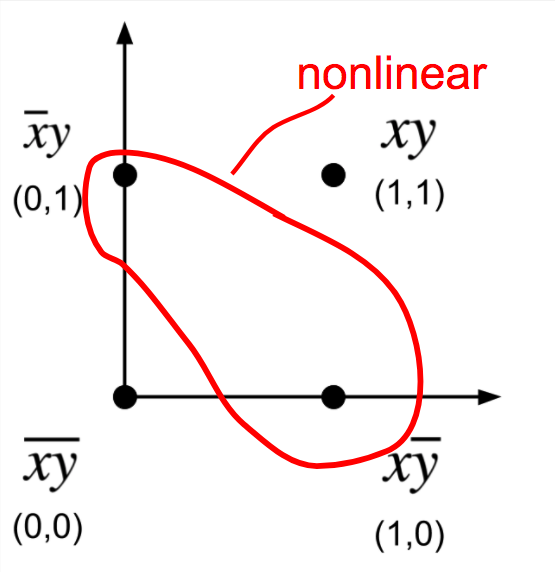
\includegraphics[width=0.3\textwidth]{papers/ableitung/images/xor_surface.png}
	\caption{Visualisierung der Punkt in einer xy-Ebene und deren separierbarkeit.}
	\label{ableitung:fig:visualisation-surface}
\end{figure}
Das Experiment wurde basierend auf dem PyTorch Framework implementiert. Das Netzwerk wurde jeweils mit der Finiten Differenzen Methode und dem Backpropagation Algorithmus trainiert. Bei der FDM wurden verschiedene Anzahl an Stützstellen (Support) gewählt und unterschiedliche Abstände $h$ verwendet. Die Resultate sind in den Abbildungen \ref{ableitung:fig:xor_h1}, \ref{ableitung:fig:xor_h01}, \ref{ableitung:fig:xor_h1} zu finden. Die y-Achse in der Abbildung stellt den quadratischen Fehler zwischen $\hat{y}$ und $y$ dar, während die x-Achse die Entwicklung über die Anzahl Iterationen aufzeigt.

\begin{figure}
	\begin{tikzpicture}
	\begin{semilogyaxis}[xmin=0, xmax=1000, ymin=10e-15, ymax=10, width=\textwidth, height=0.30\textheight]
	\addplot[one, line width=1pt] table [x=epoch, mark=none, y=loss, col sep=comma] {papers/ableitung/data/backprop.csv};
	\addplot[two] table [x=epoch, mark=none, y=loss, col sep=comma] {papers/ableitung/data/h1-support2.csv};
	\addplot[three] table [x=epoch, mark=none, y=loss, col sep=comma] {papers/ableitung/data/h1-support4.csv};
	\addplot[four] table [x=epoch, mark=none, y=loss, col sep=comma] {papers/ableitung/data/h1-support6.csv};
	\addplot[five] table [x=epoch, mark=none, y=loss, col sep=comma] {papers/ableitung/data/h1-support8.csv};
	
	\addlegendentry{Backprop}	
	\addlegendentry{Support: 2}
	\addlegendentry{Support: 4}
	\addlegendentry{Support: 6}
	\addlegendentry{Support: 8}
	
	
	\end{semilogyaxis}
	\end{tikzpicture}
	\caption{Resultate des Gradientenabstiegs mit Stützstellenabstand $h=1$.}
	\label{ableitung:fig:xor_h1}
\end{figure}

\begin{figure}	
	\begin{tikzpicture}
	\begin{semilogyaxis}[xmin=0, xmax=1000, ymin=10e-15, ymax=10, width=\textwidth, height=0.3\textheight]
	\addplot[one, line width=1pt] table [x=epoch, mark=none, y=loss, col sep=comma] {papers/ableitung/data/backprop.csv};
	\addplot[two] table [x=epoch, mark=none, y=loss, col sep=comma] {papers/ableitung/data/h01-support2.csv};
	\addplot[three] table [x=epoch, mark=none, y=loss, col sep=comma] {papers/ableitung/data/h01-support4.csv};
	\addplot[four] table [x=epoch, mark=none, y=loss, col sep=comma] {papers/ableitung/data/h01-support6.csv};
	\addplot[five] table [x=epoch, mark=none, y=loss, col sep=comma] {papers/ableitung/data/h01-support8.csv};
	
	\addlegendentry{Backprop}	
	\addlegendentry{Support: 2}
	\addlegendentry{Support: 4}
	\addlegendentry{Support: 6}
	\addlegendentry{Support: 8}
	
	
	\end{semilogyaxis}
	\end{tikzpicture}
	\caption{Resultate des Gradientenabstiegs mit Stützstellenabstand $h=0.1$.}
	\label{ableitung:fig:xor_h01}
\end{figure}
	
\begin{figure}
	\begin{tikzpicture}
	\begin{semilogyaxis}[xmin=0, xmax=1000, ymin=10e-15, ymax=10, width=\textwidth, height=0.3\textheight]
	\addplot[one, line width=1pt] table [x=epoch, mark=none, y=loss, col sep=comma] {papers/ableitung/data/backprop.csv};
	\addplot[two] table [x=epoch, mark=none, y=loss, col sep=comma] {papers/ableitung/data/h001-support2.csv};
	\addplot[three] table [x=epoch, mark=none, y=loss, col sep=comma] {papers/ableitung/data/h001-support4.csv};
	\addplot[four] table [x=epoch, mark=none, y=loss, col sep=comma] {papers/ableitung/data/h001-support6.csv};
	\addplot[five] table [x=epoch, mark=none, y=loss, col sep=comma] {papers/ableitung/data/h001-support8.csv};
	
	\addlegendentry{Backprop}	
	\addlegendentry{Support: 2}
	\addlegendentry{Support: 4}
	\addlegendentry{Support: 6}
	\addlegendentry{Support: 8}
	
	
	\end{semilogyaxis}
	\end{tikzpicture}
	\caption{Resultate des Gradientenabstiegs mit Stützstellenabstand $h=0.01$.}
		\label{ableitung:fig:xor_h001}
\end{figure}

Es ist erstaunlich, dass bereits bei diesem kleinen Netzwerk numerische Effekte im Backpropagation Algorithmus in einem etwas höheren Fehler resultieren. Der Fehler von $\approx 10^-14$ im besten Fall (FDM) ist um Faktor $10^3$ kleiner als die des Backpropagation Algorithmus.
	